% =====================================================================
%  supervisor_draft.tex
%  Decomposing Recoverability: Minimal Co-Deletion for the Right to be
%  Forgotten in LLM Agent Memory
%
%  AAAI-grade discussion draft. Self-contained: compiles with a standard
%  TeX Live install (no aaai25.sty required). Styled to read as a venue
%  submission; page/format limits are intentionally NOT enforced here and
%  will be tightened for camera-ready.
%
%  Build:  pdflatex supervisor_draft  &&  bibtex supervisor_draft  &&
%          pdflatex supervisor_draft  &&  pdflatex supervisor_draft
% =====================================================================
\documentclass[10pt,twocolumn,letterpaper]{article}

% ---- packages ---------------------------------------------------------------
\usepackage[T1]{fontenc}
\usepackage[utf8]{inputenc}
\usepackage{times}
\usepackage{microtype}
\usepackage{graphicx}
\usepackage{booktabs}
\usepackage{amsmath,amssymb,amsthm}
\usepackage{mathtools}
\usepackage{tikz}
\usetikzlibrary{positioning, arrows.meta}
\usepackage{xcolor}
\usepackage[hyphens]{url}
\usepackage[numbers,sort&compress]{natbib}
\usepackage{caption}
\usepackage{abstract}
\usepackage[margin=0.75in]{geometry}
\usepackage{titlesec}
\usepackage[colorlinks=true,allcolors=blue!55!black,breaklinks=true]{hyperref}

% ---- layout polish ----------------------------------------------------------
\setlength{\columnsep}{0.28in}
\captionsetup{font=small,labelfont=bf,skip=5pt}
\titleformat{\section}{\large\bfseries\raggedright}{\thesection}{0.6em}{}
\titleformat{\subsection}{\normalsize\bfseries\raggedright}{\thesubsection}{0.5em}{}
\titlespacing*{\section}{0pt}{1.4ex plus .3ex}{0.8ex}
\titlespacing*{\subsection}{0pt}{1.1ex plus .2ex}{0.5ex}
\renewcommand{\abstractnamefont}{\normalfont\bfseries}
\renewcommand{\abstracttextfont}{\normalfont\small}

% ---- theorem-like environments ---------------------------------------------
\theoremstyle{definition}
\newtheorem{definition}{Definition}
\newtheorem{problem}{Problem}
\theoremstyle{plain}
\newtheorem{proposition}{Proposition}
\newtheorem{remark}{Remark}

% ---- notation shorthands ----------------------------------------------------
\newcommand{\sres}{\sigma_{\mathrm{res}}}
\newcommand{\sred}{\sigma_{\mathrm{red}}}
\newcommand{\Rec}{R}
\newcommand{\Adv}{\mathcal{A}}
\newcommand{\code}[1]{\texttt{#1}}
\newcommand{\sys}[1]{\textsc{#1}}

% =============================================================================
\title{\vspace{-2.2em}\bfseries
  Decomposing Recoverability: Minimal Co-Deletion for the\\[2pt]
  Right to be Forgotten in LLM Agent Memory}

\author{
  \textbf{Muhammad Salman Al Farisi}\\[2pt]
  School of Computing, National University of Singapore\\
  Advisor: Tan Tian Huat\\
  \texttt{salman26080@gmail.com}
}
\date{}

% =============================================================================
\begin{document}
\twocolumn[
  \begin{@twocolumnfalse}
    \maketitle
    \begin{onecolabstract}
      \noindent Ask a paging LLM agent to forget a fact and it may scrub the
      working-memory block it reasons over while silently leaving the fact in
      its archival store: the deletion is acknowledged, looks complete, and is
      not. More generally, deleting a fact from an LLM agent's memory does not
      mean the agent has forgotten it. Existing audits check whether a forget
      command removes a value from retrieval, which is \emph{necessary but not
      sufficient}, because the value can persist in a derived artifact or be
      re-derived from facts that were never deleted. We formalize
      \emph{deletion-completeness} for agent memory, decomposing post-deletion
      recoverability into three causally distinct channels---residual survival,
      re-derivation from surviving facts, and a parametric floor recoverable
      from the base model alone---and give a planner that computes the minimal
      co-deletion closing the deletable channels, emitting an auditable
      certificate. Because the parametric floor cannot be deleted, certification
      has a hard limit: under the strongest modeled adversary, \textbf{23 of 49}
      facts cannot be certified erased at threshold $\tau{=}0.1$, even with
      zero residual survival and no helpful co-deletion. The same stack, run
      across three memory architectures (a deduplication pipeline, a bi-temporal
      knowledge graph, and a paging agent), finds residual survival in all three
      through different by-design mechanisms: the gap is a property of how agent
      memory derives and retains facts, not of any single system.
      \vspace{1.0em}
    \end{onecolabstract}
  \end{@twocolumnfalse}
]

% =============================================================================
\section{Introduction}\label{sec:intro}

A user invokes their right to be forgotten and asks an LLM agent to delete their
home address. A modern agent with long-term memory---a paging architecture such
as MemGPT/Letta \citep{packer2024memgpt}---acknowledges and rewrites the
working-memory block it is currently reasoning over. But the address was also
written to the agent's archival vector store in an earlier session; reasoning
only over its working context, the agent never touches it, and weeks later an
ordinary retrieval surfaces the address again. The deletion was confirmed, looked
complete, and was not.

This is not a one-off bug. Even a \emph{faithful} delete of a record need not
erase the fact it carried: the fact can survive in a derived artifact the system
built from it---a duplicate, a summary, a consolidated note---or be re-derived
from facts that remain, such as a salary from a job title plus a public pay band,
or a diagnosis from stored symptoms. The most thorough current audits of agent
forgetting \citep{forgeteval} check whether a forget command removes a value from
top-$k$ retrieval. That check is \emph{necessary but not sufficient}: it does not
ask \emph{why} a deleted fact returns, nor \emph{what minimal further deletion}
would actually close the leak. Those two questions are the subject of this paper,
and they matter directly for compliance: the GDPR right to erasure
\citep{gdpr2016} is a guarantee about a \emph{fact}, not about a row.

We cast deletion-completeness as whether a deleted fact remains recoverable, and
decompose recoverability into three causally distinct channels: residual survival
(a surviving artifact still contains the value), re-derivation (surviving facts
entail it), and a parametric floor (the base model recovers it from world
knowledge alone). The first two are closable by deleting more; the third is not.
A greedy planner computes the minimal additional co-deletion that closes the
closable channels, and a certificate records what deletion achieved, at what
collateral cost, and---crucially---when the parametric floor makes erasure
impossible to certify. Concretely, we contribute:

\begin{itemize}\itemsep2pt
  \item A formal, \emph{adversary-relative} deletion-completeness criterion for
    agent memory, strictly stronger than dependency-bounded database erasure,
    decomposing recoverability into residual, re-derivation, and parametric
    channels (\S\ref{sec:formulation}).

  \item A minimal co-deletion planner for the resulting NP-hard problem, reaching
    completeness at mean collateral $k=0.91$ with zero spurious deletions, plus an
    auditable certificate that separates what deletion achieved from what it
    cannot (\S\ref{sec:method}, \S\ref{sec:res-planner}).

  \item A \emph{measured} parametric floor and its limit result: under the
    strongest modeled adversary, $23/49$ facts cannot be certified erased even at
    zero residual survival---a measured gradient in which the threshold $\tau$ is a
    deliberate policy dial (\S\ref{sec:res-rho}).

  \item Evidence of generality: the same probe/planner/certificate stack, run on
    three memory architectures, exposes residual survival in all three through
    different by-design mechanisms, including the agent-loop failure above that
    prior audits bypass (\S\ref{sec:res-converge}).
\end{itemize}

The breadth across systems is evidence for a stronger, causally-decomposed notion
of erasure---not a claim to be first to evaluate these systems, since ForgetEval
\citep{forgeteval} already benchmarks all three, but a stronger question asked of
them. What is new is asking, and answering, why deleted facts return and what it
costs to make them stay gone.

% =============================================================================
\section{Related Work}\label{sec:related}

\paragraph{Auditing forgetting in agent memory.}
The closest prior work is \sys{ForgetEval} \citep{forgeteval}, the most thorough
existing audit of forgetting in deployed agent memory---a careful retrieval-based
protocol spanning Mem0 \citep{mem0}, Graphiti/Zep \citep{rasmussen2025zep},
Letta \citep{packer2024memgpt}, and roughly a dozen further systems---and we build
directly on it. Its retrieval-based criterion is the \emph{necessary-but-not-
sufficient} gap of \S\ref{sec:intro}. Our contribution is therefore the stronger,
channel-decomposed criterion, not the system coverage ForgetEval already
establishes; correspondingly, our Mem0 figures (recoverability by \emph{any}
channel) are complementary to its top-$k$ forget-command rates, not in tension
with them. Two of our results extend it directly. ForgetEval deliberately bypasses
Letta's agent loop---addressing archival endpoints to keep the model out of the
recall path---which is exactly the loop we exercise and find surface-incomplete
(\S\ref{sec:res-converge}); and its own per-system observations (Graphiti shedding
synthesized fact strings, Mem0's router favoring link-and-keep) name the
mechanisms our decomposition isolates, independently corroborating the convergence
result.

\paragraph{Unlearning methods.}
\sys{Agentic Unlearning} \citep{agenticunlearning} separates parametric from
memory recovery (its ``backflow''), but assumes \emph{weight access} to edit the
model; we operate black-box and memory-store-only, so we neither claim the
parametric/memory split as novel nor perform model surgery. More broadly, the
machine-unlearning line---exact and approximate forgetting of training data
\citep{cao2015towards,bourtoule2021unlearning,nguyen2022survey}---targets a
\emph{parametric} object (knowledge in weights). Our object is orthogonal and
black-box: an external memory store and what an adversary can reconstruct from its
\emph{surviving} contents. The two meet only at the parametric floor $\rho$, which
we measure but cannot remove without exactly the weight access we forgo.

\paragraph{Deletion under dependencies.}
Our formal grounding is the database line on erasure when records are
inter-derivable: P2E2's meaningful-erasure criterion \citep{p2e2} and
inference-aware deletion \citep{seqdb}. We port P2E2's \emph{dependency-bounded}
criterion to agent memory and deliberately \emph{strengthen} it---its baseline
keeps pre-existing operands present, which is vacuous for the right to be
forgotten---while inheriting its NP-hardness via classical hitting-set/vertex-cover
hardness \citep{karp1972reducibility,garey1979computers}. This bridge, from
relational deletion theory to LLM agent memory, is one the agent-memory works
above do not make.

\paragraph{Memory evaluation and LLM judges.}
Memory benchmarks largely score \emph{retrieval} quality
\citep{maharana2024locomo,wu2025longmemeval}; we instead score \emph{adversarial
recoverability after deletion}, and we treat our LLM judges as load-bearing
instruments to be validated rather than trusted. LLM-as-judge is known to be
biased and miscalibrated \citep{zheng2023judge,sharma2024sycophancy}, and label
noise destabilizes benchmark conclusions \citep{northcutt2021labelerrors}; we
therefore report a false-accept rate against gold for the recovery judge and
inter-judge agreement on hard negatives for the entailment judge
(\S\ref{sec:res-judge}), so every recovery rate we report is a conservative lower
bound rather than a judge artifact.

% =============================================================================
\section{Problem Formulation}\label{sec:formulation}

\paragraph{Setup.}
Let $f$ be a target fact with value $v$ and let $\Sigma(v)$ be its set of
ground-truth surface forms. A memory store $S$ is a set of records; a deletion
operation yields a surviving store $S'\subseteq S$. The adversary $\Adv$ has full
read access to $S'$, black-box access to a base model $M$, and general world
knowledge $W$; a query $q_f$ asks for $v$. Write $\mathrm{rec}(a)=1$ iff answer
$a$ reveals a surface form in $\Sigma(v)$ (within the stated value), as scored by
the validated recovery judge (\S\ref{sec:res-judge}). Two of the three channels
below depend on $\Adv$'s reasoning model, so recoverability is
\emph{adversary-relative} (Definition~\ref{def:rec}).

\begin{definition}[Residual survival]\label{def:res}
$\;\sres(f,S')=\mathbb{1}\!\left[\exists\, r\in S':\;\Sigma(v)\cap\mathrm{txt}(r)\neq\emptyset\right].$
A surviving record physically contains the value.
\end{definition}

\begin{definition}[Re-derivation]\label{def:red}
$\;\sred^{\Adv}(f,S')=\mathrm{rec}\!\left(\Adv(q_f \mid S',M,W)\right).$
The adversary reconstructs $v$ by reasoning over the \emph{surviving store} plus
world knowledge.
\end{definition}

\begin{definition}[Parametric floor]\label{def:rho}
$\;\rho^{\Adv}(f)=\mathrm{rec}\!\left(\Adv(q_f \mid \emptyset, M, C)\right),$
where $C\subseteq W$ is the subject's world-knowable context and the store is
\emph{empty}. $\rho^{\Adv}$ has no dependence on $S$ and is therefore
\emph{system-independent}; we estimate it as a recovery rate over stochastic
samples.
\end{definition}

\begin{definition}[Recoverability, adversary-relative]\label{def:rec}
$\;\Rec_{\Adv}(f,S')=\max\!\left(\sres,\;\sred^{\Adv},\;\rho^{\Adv}\right).$
\end{definition}

The $\max$ is the worst-case-channel principle: one open channel suffices, so a
rational adversary uses whichever is open. True recoverability is
$\sup_{\Adv}\Rec_{\Adv}$; we bracket it with two concrete adversaries,
$\Adv_{\text{mini}}$ (\code{gpt-4o-mini}) and $\Adv_{4o}$ (\code{gpt-4o}), so the
two per-reasoner values of $\rho$ are principled points bracketing the floor.

\begin{definition}[Floor-reaching and erasure-certification]\label{def:cert}
A deletion is \textbf{floor-reaching} for $\Adv$ iff $\sres=\sred^{\Adv}=0$
---recoverability is driven to the parametric floor and nothing further is
deletable---and \textbf{erasure-certified} iff it is floor-reaching for every
modeled adversary and additionally
$\sup_{\Adv}\Rec_{\Adv}(f,S')=\max_{\Adv}\rho^{\Adv}<\tau$.
\end{definition}

\paragraph{Stronger than P2E2 (and why).}
This criterion is deliberately \emph{stronger} than the dependency-bounded erasure
of \citet{p2e2}, whose baseline keeps pre-existing operands present; under it,
deleting $f$'s own records already suffices even when $f$ re-derives from surviving
independent operands, so our operand co-deletion would count as over-deletion. We
reject that baseline as \emph{vacuous for the right to be forgotten}: a diagnosis
still re-inferable from stored symptoms has not been forgotten. We therefore set
the baseline at $\rho^{\Adv}$ (world knowledge only, every stored operand removed).

\begin{remark}[The limit result]\label{rmk:limit}
Floor-reaching is \emph{always} achievable by co-deletion; erasure-certification
fails exactly when $\rho^{\Adv}\geq\tau$, because $\rho$ has no store dependence
and no co-deletion can lower it. The certificate then reports \emph{floor-reaching
but not erasure-certified} even at $\sres=\sred=0$: the fact is as erased as
deletion can make it, yet remains world-inferable.
\end{remark}

\begin{remark}[The residual--floor boundary]\label{rmk:boundary}
If $v$ is pinned by a stored operand $o\in S'$, the recovery is re-derivation
($\sred$) and is removable by co-deleting $o$; if $v$ is pinned by world-knowable
context $C\subseteq W$, the recovery is parametric ($\rho$) and is \emph{not}
removable.
\end{remark}

\begin{remark}[Over-deletion is the measured price of erasure]\label{rmk:price}
Co-deleting un-requested entailers is the \emph{measured, minimized} cost---the
collateral $k$---of an actual erasure guarantee, because leaving them is not
minimization but \emph{failed} erasure. The planner minimizes $k$, the floor
$\rho$ bounds what no deletion can remove, and the certificate surfaces $k$.
\end{remark}

\paragraph{The optimization problem (Opt-P2E2).}
Let $R_f\subseteq S$ be $f$'s own records. We seek the minimal-collateral
co-deletion making $f$ floor-reaching:
\begin{equation}
  \min_{D\,\subseteq\, S\setminus R_f} |D|
  \quad\text{s.t.}\quad
  \sred^{\Adv}\!\left(f,\; S\setminus(R_f\cup D)\right) = 0 .
\end{equation}

\begin{proposition}[NP-hardness]\label{prop:nphard}
\textsc{Opt-P2E2} is NP-hard, by reduction from \textsc{Minimum Hitting Set}.
\end{proposition}
\begin{proof}[Proof sketch]
Given a universe $U$ and sets $\mathcal{S}=\{S_1,\dots,S_m\}$ with
$S_j\subseteq U$, construct an instance with one fact $x_u$ per element $u\in U$
and, for each $S_j$, an entailment $\bigwedge_{u\in S_j} x_u \vdash f$ (so each
$S_j$ is a re-derivation path). The surviving store re-derives $f$ iff some path
$S_j$ survives intact, so a co-deletion $D$ achieves $\sred=0$ iff
$D\cap S_j\neq\varnothing$ for every $j$---i.e.\ $\{u:x_u\in D\}$ is a hitting set
of $\mathcal{S}$. Thus $\min|D|$ equals the minimum hitting set
\citep{karp1972reducibility}. \textsc{Vertex Cover} is the $2$-uniform special
case, which is exactly our dataset's pairwise-entailment regime: hardness already
holds when every fact has exactly two operands. We therefore adopt a greedy,
entailment-confidence-ordered planner (\S\ref{sec:method}).
\end{proof}

% =============================================================================
\section{Method}\label{sec:method}

Our pipeline instantiates each object of \S\ref{sec:formulation} as a concrete,
reusable component behind a single \code{MemorySystemAdapter} interface, so the
identical probe/planner/certificate stack runs unchanged on all three systems.

\paragraph{Probe battery.}
Three probes measure the three channels of Definition~\ref{def:rec}. The
\emph{exact-match} probe scans every surviving record for a surface form of $v$
($\sres$). The \emph{re-derivation} probe gives the adversary the full surviving
store as notes (plus today's date and general world knowledge) and elicits $v$ in
a value-first format ($\sred^{\Adv}$). The \emph{parametric} probe withholds the
store entirely, conditioning only on the subject's world-knowable context, and
estimates $\rho^{\Adv}$ as a recovery rate over $n$ stochastic samples. Recovery
is decided by the validated judge (\S\ref{sec:res-judge}): a substring match on
the ground-truth surface forms, falling back to an LLM adjudication for
numeric/semantic approximation. Three auxiliary probes support specific
results---a \emph{paraphrase} probe (residual by implication), a retrieval-score
\emph{membership-inference} probe (\S\ref{sec:limitations}), and a \emph{KG-summary}
probe for the graph system (\S\ref{sec:res-converge}).

\paragraph{Entailment detector.}
Re-derivation paths are found by an LLM-as-judge that scores, for a candidate
surviving fact (or set), the confidence that it entails $v$ given world knowledge,
returning a value in $[0,1]$. The detector both draws the dependency edges and
orders co-deletion. Its validation (\S\ref{sec:res-judge}) dictates the choice of
\code{gpt-4o} here, since a judge that false-fires on partial operands inflates the
collateral.

\paragraph{Co-deletion planner.}
Against a \emph{naive} baseline that deletes only the single surfaced record (no
co-deletion), we implement two co-deletion heuristics. \emph{Threshold} (the
method) probes, purges the target's own artifacts using the narrow deletion
surface form, then co-deletes entailing facts in descending entailment confidence,
re-probing after each until $\sred^{\Adv}<\tau$---making $f$ floor-reaching with a
greedily minimal $D$. \emph{Depth-first} (an aggressive comparator) co-deletes
every entailer above $\tau$ in one shot, with no re-probe stopping rule. The
reported collateral $k=|D|$ is the measured price of the strong erasure notion;
the threshold heuristic minimizes it ($k=0.91$ vs.\ depth-first's $5.65$,
\S\ref{sec:res-planner}).

\paragraph{Certificate emitter.}
For each target the emitter records the three channel scores, the final
recoverability $\Rec_{\Adv}=\max(\cdot)$, the heuristic, the co-deleted set and its
size $k$, and the threat model. It exposes two machine-readable predicates from
Definition~\ref{def:cert}: \code{floor\_reaching} (the deletable channels closed)
and \code{completeness\_certified}. The latter certifies erasure only under the
\emph{worst modeled adversary}---$\rho=\max_{\Adv}\rho^{\Adv}<\tau$---so a fact
recoverable by the stronger reasoner is reported uncertified even when the weaker
one fails; this conservative choice is why $23/49$, not $14/49$, are uncertifiable
(\S\ref{sec:res-rho}).

% =============================================================================
\section{Experiments}\label{sec:results}

We evaluate on three deployed agent-memory systems spanning three architecture
families: \textbf{Mem0} (\code{mem0ai} 2.0.7, a deduplicating extraction pipeline
over local Chroma; \citealp{mem0}), \textbf{Zep/Graphiti} (\code{graphiti-core}
0.29.2, a bi-temporal knowledge graph over Neo4j~5.26; \citealp{rasmussen2025zep}),
and \textbf{Letta/MemGPT} (\code{letta}~0.16.8, an LLM-paging agent over Postgres +
pgvector; \citealp{packer2024memgpt}). Every component runs locally with pinned
versions and disabled telemetry, so the pipeline is reproducible from a clean
checkout. The deletion adversary has full read access to the surviving store and
black-box access to the base model. Two pinned reasoners are used wherever recovery
is model-dependent: \code{gpt-4o-mini-2024-07-18} (primary) and
\code{gpt-4o-2024-08-06}; embeddings are local \code{all-MiniLM-L6-v2}. The
completeness threshold is $\tau=0.10$. Datasets are synthetic subjects placed in
realistic statistical contexts: 48 isolated PII facts, 34 multi-hop facts with their
stored operands and bystanders, and 49 parametric-gradient facts across three
difficulty tiers. Recovery is scored by a validated LLM judge with no observed
false accepts (\S\ref{sec:res-judge}: $0/8$ gold negatives), so every reported
recovery rate is a conservative lower bound. Table~\ref{tab:master} summarizes the
headline numbers, ordered by confidence.

\begin{table*}[t]
\centering
\small
\begin{tabular}{@{}llll@{}}
\toprule
\textbf{Result} & \textbf{System} & \textbf{Headline} & \textbf{Backing control} \\
\midrule
Planner (\S\ref{sec:res-planner})     & Mem0          & 100\% complete, 0 spurious, $k{=}0.91$ & spare-bystander + gpt-4o entailment \\
$\rho$ floor (\S\ref{sec:res-rho})    & base model    & 23/49 \emph{uncertifiable} at residual~0 & worst-adversary $\rho$; refusal audit \\
Re-derivation (\S\ref{sec:res-rederiv}) & Mem0, Letta & bin1 100\%, bin2 59--65\%$\to$0\%       & operands-only; faithful co-delete \\
Convergence (\S\ref{sec:res-converge}) & all three    & 80\% / 100\% (Graphiti/Letta)          & clean-delete verified first \\
Residual (\S\ref{sec:res-residual})   & Mem0          & 97.9\%; 68.75\%$\to$0\%                 & $2{\times}2$ embedder$\times$cadence factorial \\
Judge (\S\ref{sec:res-judge})         & ---           & $0/8$ false-accept                     & gold set + 12 hard near-miss negatives \\
\bottomrule
\end{tabular}
\caption{Headline results, ordered by confidence. Each row's claim is admitted
only because the named control rules out the obvious confound. $\rho$ is measured
world-context-only against the base model and is therefore system-independent.}
\label{tab:master}
\end{table*}

% ---------------------------------------------------------------------------
\subsection{Minimal Co-Deletion: The Planner}\label{sec:res-planner}

On the full 34 multi-hop targets, the threshold planner achieves \textbf{100\%
completeness} (Wilson $[0.90,1.0]$) \textbf{with 0 spurious bystander deletions} and
a \textbf{mean collateral of $k=0.91$} (bootstrap $[0.74,1.09]$); minimality spares
36 operands whose deletion was unnecessary once a sufficient subset was removed.

\textbf{Control.} The 0-spurious figure is the selectivity test: the candidate pool
mixes true operands with bystanders the planner must not touch. The result is
robust to the entailment judge: re-running with the stronger \code{gpt-4o} judge
leaves completeness, spurious count, and $k$ unchanged. This robustness is not
incidental---our entailment-judge validation (\S\ref{sec:res-judge}) shows
\code{gpt-4o-mini} false-fires on $41.7\%$ of \emph{insufficient} partial operands
while \code{gpt-4o} false-fires on $0\%$, so using \code{gpt-4o} is precisely what
prevents $k$ from inflating.

\textbf{Comparator.} Depth-first guarantees floor-reaching without iterative
probing---one pass co-deleting every entailer above $\tau$---and reaches $100\%$
completeness at $k=5.65$ (with $126$ spurious bystander deletions). Threshold attains
the \emph{same} completeness at $k=0.91$: iterative re-probing converts that
guarantee into a $\sim6\times$ reduction in collateral ($5.65\to0.91$) and full
selectivity ($126\to 0$ spurious).

\begin{table}[t]
\centering
\small
\begin{tabular}{@{}lcc@{}}
\toprule
Field & \textsc{complete} & \textsc{incomplete} \\
\midrule
Example (system)                       & F040 (Letta)  & R11 (Mem0) \\
\code{residual\_survival}              & 0.0           & 0.0 \\
\code{rederiv\_with\_operands} (pre)   & 1.0           & --- \\
\code{re\_derivation\_score} (final)   & 0.0           & 0.0 \\
\code{parametric\_risk\_rho}           & 0.0           & \textbf{1.0} \\
\code{facts\_co\_deleted} ($k$)        & C001,C002 (2) & --- (0) \\
\code{final\_recoverability}           & 0.0           & 1.0 \\
\code{floor\_reaching}                 & true          & \textbf{true} \\
\code{completeness\_certified}         & \textbf{true} & \textbf{false} \\
\bottomrule
\end{tabular}
\caption{Two representative certificates. \emph{Left:} the re-derivation channel
was open before co-deletion and closed after, giving \textsc{complete}.
\emph{Right:} residual and re-derivation are both $0$, but the system-independent
base-model floor $\rho{=}1.0$ forces \textsc{incomplete}. Both are
\code{floor\_reaching} (deletion did its job); only the left is
\code{completeness\_certified}---the right is the limit result.}
\label{tab:certs}
\end{table}

% ---------------------------------------------------------------------------
\subsection{The Parametric Floor and the Limit of Certifiable Deletion}
\label{sec:res-rho}

We \emph{measure} the parametric floor $\rho$---the rate at which the base model
alone reconstructs a value from world-knowable context---rather than asserting it.
We report by the $\rho$ we \emph{measure}, not the authored tier: the two disagree
for $16/49$ facts, which we retain and report by measured $\rho$ rather than
discard---authored tiers are hypotheses, measured $\rho$ is the evidence. The
worst-adversary $\rho_{\max}{=}\max_\Adv\rho^\Adv$ splits the set into \textbf{26 at
$\rho_{\max}{\le}\tau$} (certifiable), \textbf{14 at $\rho_{\max}{\ge}0.5$} (a hard
floor), and \textbf{9 in an intermediate band} (Table~\ref{tab:rho}). By authored
tier the means are (\code{gpt-4o-mini}\,/\,\code{gpt-4o}) \textbf{low $0.00/0.00$},
\textbf{mid $0.069/0.265$}, \textbf{high $0.367/0.656$}.

Certifying erasure under the \emph{worst} modeled adversary, \textbf{23 of 49
certificates are \emph{not} erasure-certifiable} at $\tau{=}0.1$ ($\rho_{\max}>\tau$)
\emph{even though residual survival is $0$}; under the weaker reasoner alone only
$14/49$ would be flagged. That eight-certificate gap is Definition~\ref{def:rec}'s
\emph{adversary-relative} recoverability made concrete: a weaker-reasoner attacker
would wrongly certify eight facts the stronger adversary recovers, so certifying
under the $\sup$ is the conservative choice a privacy certificate must make.

The worst-adversary $\rho$ forms a \emph{measured gradient} of parametric
recoverability---from 26 facts at the certifiable floor, through 8 in an
intermediate band, to 14 at a hard floor---rather than an all-or-nothing split.
Because the floor is graded, the uncertifiable count is genuinely
\emph{threshold-dependent} ($22$ at $\tau{=}0.1$, falling to $14$ as
$\tau\!\to\!0.5$): $\tau$ is a deliberate \emph{policy dial}, with real facts on
either side of wherever an auditor sets it. This is the limit result: when the
value is recoverable from non-deletable world knowledge, no co-deletion can
certify erasure.

\textbf{Control.} The $\rho$ probe sees \emph{only} the subject's world-knowable
context, never the stored facts, so co-deletion provably cannot lower it. Three
hardening checks back the gradient: a mid-tier numeric-tolerance sweep shows the
floor persists at every tolerance; a base-rate vs.\ context-lift split separates
genuine inference from prior plausibility; and a high-tier refusal audit (R13,
refused on $5/6$ samples by \code{gpt-4o-mini}) means $\rho$ for sensitive
attributes is an \emph{adversarial lower bound}.

\begin{table}[t]
\centering
\small
\begin{tabular}{@{}lcc@{}}
\toprule
measured worst-adversary band & \#facts ($n{=}49$) & certifiable \\
\midrule
$\rho_{\max}\le\tau$ ($\tau{=}0.1$; certifiable floor) & 26 & 26 \\
$\tau<\rho_{\max}<0.5$ (intermediate band)            & 9  & 0  \\
$\rho_{\max}\ge0.5$ (hard floor)                      & 14 & 0  \\
\midrule
total                                                 & 49 & 26 \\
\bottomrule
\end{tabular}
\caption{Parametric floor $\rho$ on $n{=}49$ facts ($6$ samples each, temperature
$0.7$), binned by the \emph{measured} worst adversary
$\rho_{\max}{=}\max(\rho_{\text{mini}},\rho_{4o})$. 26 facts sit at the certifiable
floor ($\rho_{\max}{\le}\tau$), 14 at a hard floor, and 9 in an intermediate
band---a graded floor, so the $23/49$ uncertifiable count is threshold-dependent
($22$ at $\tau{=}0.1$, $14$ as $\tau\!\to\!0.5$). Authored tier disagrees with the
measured band for $16/49$ facts; authored-tier means $0.00/0.00$ (low),
$0.069/0.265$ (mid), $0.367/0.656$ (high) (\code{mini}/\code{4o}).}
\label{tab:rho}
\end{table}

% ---------------------------------------------------------------------------
\subsection{Decomposing Recovery: Re-Derivation at Zero Residual}
\label{sec:res-rederiv}

Using an operands-only control---the post-deletion state in which the target's own
value is never stored, so residual survival is $0$ by construction---we isolate the
re-derivation channel. On Mem0, the leak is \textbf{100\%/94\% for stored-alone (bin~1)
and $59\%/65\%$ for stored+world (bin~2)} (\code{gpt-4o-mini}/\code{gpt-4o}, $n{=}17$
per bin), collapsing to \textbf{$0\%$ after co-deleting the operands}, with
parametric floor $\rho=0\%$.
The same control \textbf{ports unchanged to Letta}: bin~1 $100\%$, bin~2 $80\%$
(\code{gpt-4o-mini})\,/\,$100\%$ (\code{gpt-4o}), again $\to 0\%$ after
co-deletion. The lone bin~2 fact separating the two reasoners on Letta is F043 (the
Catholic High School $\to$ Bishan geographic leap), which does not leak on Mem0
under either reasoner; on Letta the adversary's notes also include the agent's core
identity block, and that extra context tips this single borderline inference for
the stronger reasoner---a system-mediated difference, not a contradiction.

\textbf{Control.} Recovery is binned by mechanism and never aggregated across bins,
and run on two reasoners, because re-derivation is model-dependent. Crucially, on
Letta the co-deletion is issued through the \emph{direct, deterministic}
\code{passages.delete} (by captured passage id), not a conversational request, and
we verify every operand passage is gone: faithful co-deletion $=100\%$, bystanders
intact $=100\%$. ``Re-derivation closed'' therefore cannot be confounded with ``the
delete silently did not execute.''

% ---------------------------------------------------------------------------
\subsection{Generalization: Three Families, One Phenomenon}
\label{sec:res-converge}

\begin{figure}[t]
\centering
\resizebox{\columnwidth}{!}{%
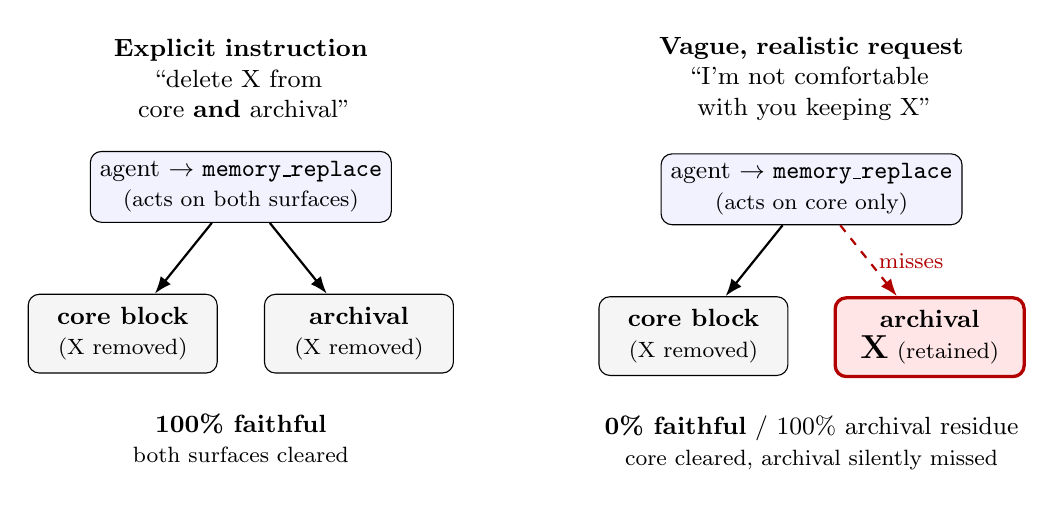
\begin{tikzpicture}[
  font=\small,
  surf/.style={rectangle, rounded corners, draw, minimum width=24mm, minimum height=10mm, align=center},
  cleared/.style={surf, fill=black!4},
  residual/.style={surf, draw=red!70!black, fill=red!10, very thick},
  agent/.style={rectangle, rounded corners, draw, fill=blue!5, minimum width=36mm, minimum height=9mm, align=center},
  instr/.style={align=center, text width=44mm},
  arr/.style={-{Latex[length=2.2mm]}, thick},
  faith/.style={align=center}
]
% ----- Panel A: explicit -----
\node[instr] (iA) {\textbf{Explicit instruction}\\``delete X from core \textbf{and} archival''};
\node[agent, below=3mm of iA] (aA) {agent $\to$ \code{memory\_replace}\\\footnotesize(acts on both surfaces)};
\node[cleared, below=9mm of aA, xshift=-15mm] (cA) {\textbf{core block}\\\footnotesize(X removed)};
\node[cleared, below=9mm of aA, xshift=15mm]  (rA) {\textbf{archival}\\\footnotesize(X removed)};
\draw[arr] (aA) -- (cA);
\draw[arr] (aA) -- (rA);
\node[faith, below=23mm of aA] {\textbf{100\% faithful}\\\footnotesize both surfaces cleared};
% ----- Panel B: vague -----
\node[instr, right=26mm of iA] (iB) {\textbf{Vague, realistic request}\\``I'm not comfortable with you keeping X''};
\node[agent, below=3mm of iB] (aB) {agent $\to$ \code{memory\_replace}\\\footnotesize(acts on core only)};
\node[cleared, below=9mm of aB, xshift=-15mm]  (cB) {\textbf{core block}\\\footnotesize(X removed)};
\node[residual, below=9mm of aB, xshift=15mm]  (rB) {\textbf{archival}\\{\large\textbf{X}}~\footnotesize(retained)};
\draw[arr] (aB) -- (cB);
\draw[arr, red!70!black, dashed] (aB) -- (rB)
  node[midway, right, red!70!black, font=\footnotesize] {misses};
\node[faith, below=23mm of aB] {\textbf{0\% faithful} / 100\% archival residue\\\footnotesize core cleared, archival silently missed};
\end{tikzpicture}}
\caption{\textbf{Same Letta agent, opposite outcomes by phrasing.} An explicit
dual-surface instruction (left) makes the agent scrub both the core block and the
archival store---$100\%$ faithful. A vague, deployment-realistic request (right)
makes the \emph{same} agent call \code{memory\_replace} on the core block it
reasons over and silently miss archival---$0\%$ faithful, $100\%$ archival residue.
The gap is phrasing and surface coverage, not capability: the explicit baseline
proves the agent \emph{can} clear both.}
\label{fig:agentloop}
\end{figure}

Residual survival is not a Mem0 quirk; it recurs across all three families by
\emph{different by-design mechanisms}. The two cross-system probes here are run on
$n{=}10$ sensitive-PII targets per system. In \textbf{Graphiti}, the explicit
\code{remove\_episode} is clean for the graph---it hard-deletes the episode, its
\code{RELATES\_TO} edges, and orphaned entities---yet the deleted fact survives in
\textbf{stale entity and community summaries that are not recomputed on deletion}:
edge residue $40\%$ but \textbf{summary residue $80\%$} (residual counts a value
present in any surviving edge or summary regardless of its bi-temporal
\texttt{invalid\_at}/\texttt{expired\_at}, consistent with the full-read-access
threat model). In \textbf{Letta},
deletion is agent-mediated across two surfaces (core blocks and archival passages).
An explicit dual-surface instruction is \textbf{$100\%$ faithful}; but a
\emph{vague, deployment-realistic} right-to-be-forgotten request with the fact also
in archival makes the agent scrub the core block it reasons about and
\textbf{silently miss archival}: \textbf{$0\%$ faithful, $100\%$ archival residue}
(Figure~\ref{fig:agentloop}).

\textbf{Novelty.} This agent-loop failure is genuinely new: ForgetEval
\citep{forgeteval} deliberately bypassed Letta's agent loop (addressing the
archival REST endpoints directly, keeping the LLM out of the recall hot path), so
we test exactly the path it excluded. ForgetEval's own per-system notes
independently corroborate our convergence thesis---its observation that Graphiti
``sheds surface forms / synthesized fact strings'' is our stale-summary residue,
and that Mem0's router prefers ``link-and-keep over delete-old'' is our duplication
residue.

\textbf{Control.} For Graphiti, verifying the clean hard delete first establishes
that the residue is stale summaries, not failed edge removal. For Letta, the
$100\%$-faithful explicit baseline isolates the failure to phrasing/surface
coverage, not to a missing capability.

% ---------------------------------------------------------------------------
\subsection{Residual Survival and the Duplication Mechanism}
\label{sec:res-residual}

Naive single-record deletion on Mem0 is residually incomplete because the store
\emph{silently duplicates} facts. Deleting the single surfaced record leaves the
value present in \textbf{$97.9\%$} of isolated PII targets ($47/48$); an
artifact-aware deletion drives residual survival from \textbf{$68.75\%$ to $0\%$}.
The two naive-arm rates ($97.9\%$ vs.\ $68.75\%$) come from separate injection runs
whose stochastic Mem0 dedup draws differ, reported as two independent measurements
of the same residual-incompleteness phenomenon.

\textbf{Control.} A $2{\times}2$ factorial over embedder (MiniLM\,/\,OpenAI)
$\times$ injection cadence ($0\,$s\,/\,$1.5\,$s) shows row-inflation of $24$--$42\%$
and duplication incidence of $30$--$39\%$ in \emph{all four} cells, with
paraphrase-variant duplicates outnumbering byte-identical ones in every cell. The
duplication is therefore a semantic-dedup \emph{design limitation}, not an artifact
of our embedder or an injection-timing race; it is independently documented in
Mem0 issues \#4896, \#4573, and \#687. These rates are not in tension with
ForgetEval's Mem0 numbers: their figure is forget-command success in top-$k$
retrieval, whereas ours is post-deletion recoverability by \emph{any}
channel---complementary measurements of necessary vs.\ sufficient conditions for
completeness.

% ---------------------------------------------------------------------------
\subsection{Judge Validation}\label{sec:res-judge}

Two LLM judges are load-bearing, so both are validated against gold labels. The
\textbf{recovery judge} produced \textbf{no false accepts} on the gold set
($n{=}17$; 7 true positives, 0 false positives, 8 true negatives, 2 false
negatives; $\kappa=0.767$ vs.\ gold). Because this rests on only $8$ negatives, the
$0$ false-accept count carries a $95\%$ Wilson upper bound of $\approx0.32$; the
lower-bound framing holds up to that bound, and its two errors are both
\emph{conservative} rejections. The \textbf{entailment judge} is validated on 24
pairs including 12 hard near-miss negatives (partial operands that should
\emph{not} entail): inter-judge agreement falls from $\kappa=0.83$ on trivial pairs
to $0.455$ on the hard near-misses, and \code{gpt-4o-mini} false-fires on $41.7\%$
of insufficient operands versus $0\%$ for \code{gpt-4o}. This is the direct
justification for using \code{gpt-4o} as the planner's entailment judge
(\S\ref{sec:res-planner}).

% =============================================================================
\section{Limitations}\label{sec:limitations}

\paragraph{A retracted---then powered---membership claim.}
An early result suggested a membership signal survived artifact-aware deletion; at
$n{=}6$ it was underpowered and we retracted it. Powered to $48$ members with two
matched near-twins each ($96$ controls), bootstrap $95\%$ CIs, and a
label-permutation test, the picture is sharp: artifact-aware deletion restores
membership-indistinguishability (AUC $0.52$, CI $[0.41,0.62]$ includes $0.5$,
$p{=}.36$), the intact store is detectable (AUC $0.69$, $p{=}.001$, so the test
\emph{has} power), and the \textbf{naive-deletion signal is now significant} (AUC
$0.68$, CI $[0.59,0.77]$ excludes $0.5$, $p{=}.001$). At this power, naive
single-record deletion \emph{does} leave a detectable membership signal; only
artifact-aware deletion removes it.

\paragraph{Judge-dependent measurements, bounded.}
Both LLM judges are validated, neither is perfect. The entailment judge's
inter-rater agreement falls to $\kappa{=}0.455$ on hard near-miss negatives, where
\code{gpt-4o-mini} false-fires on $41.7\%$; we use \code{gpt-4o} (no false-fires on
our cases) as the planner's judge. The recovery judge had no false accepts, but
over only $8$ gold negatives---a $95\%$ Wilson upper bound of $\approx0.32$.
Tightening this bound with adversarial near-miss recoveries (e.g.\ ``$\approx$3,190''
for $3{,}200$) is the most valuable validation extension.

\paragraph{$\rho$ is a lower bound where it matters most.}
The parametric floor is estimated by eliciting the value from the base model; for
sensitive attributes the model often refuses ($7$ high-tier items drew refusals), so the measured $\rho$
\emph{understates} true world-inferability for exactly the attributes a privacy
audit cares about. A more willing \emph{reasoner} could only push the uncertifiable count
above $23/49$, never below; this monotonicity is over reasoner adversaries---the
recovery judge is the single validated \texttt{gpt-4o-mini}.

\paragraph{The entailment graph must be known.}
The decomposition and planner assume the entailment graph is specified---the
operands that re-imply a fact are known, as they are in our controlled setup. In a
deployed store the graph is neither given nor easily recovered: the planner closes
only re-derivation paths through \emph{known} entailers, so an unmodeled entailer
is an uncloseable path. Discovering the entailment graph of a live memory is itself
an open problem.

\paragraph{Small cross-system samples.}
The convergence result probes $n{=}10$ high-stakes targets per system (scaled
from an initial $n{=}3$). The mechanisms are qualitatively distinct and each is
independently corroborated \citep{forgeteval}, but the per-system rates (e.g.\ $80\%$
summary residue in the graph store) remain indicative, not precise at this scale. Finally, all subjects are synthetic, so
recoveries reflect re-derivability rather than memorized real individuals, and we
model two reasoner adversaries rather than the supremum over all of them.

% =============================================================================
\section{Conclusion}\label{sec:conclusion}

Deleting a record is not erasing a fact. We gave a causal decomposition of
post-deletion recoverability, a planner that closes the deletable channels with
minimal collateral, and a certificate that states, per fact, both the cost of
erasure and whether it can be certified at all. Across three memory architectures
the same gap recurs through different by-design mechanisms, and a \emph{measured}
parametric floor sets a hard limit on what any deletion can promise.

That limit is the paper's broadest implication. For a fact recoverable from world
knowledge alone ($\rho\geq\tau$)---$23$ of our $49$ gradient facts under the
strongest modeled adversary---\emph{no} external-store deletion method can achieve
erasure, because the value can be reconstructed without ever reading the store. For
such facts, right-to-be-forgotten compliance cannot be a deletion operation: it
requires not storing the fact in the first place, or explicitly accepting and
disclosing the residual floor.

One extension is immediate: adding a fourth memory architecture to test whether
the three-family convergence is universal. The deeper
open problem is certifying erasure against an unbounded adversary rather than a
modeled bracket: the floor we measure is a lower bound, so the true limit of
forgetting in agent memory may be higher still.

% =============================================================================
\bibliographystyle{plainnat}
\bibliography{references}

\end{document}